% modo presentación. si se cambia a modo notas se imprimen las notas (creo)
\documentclass[xcolor={dvipsnames,x11names,svgnames},aspectratio=169,notes]{beamer}
\mode<presentation>
%handout de las diapositivas, comentar arriva!
% handout de la presentacion
%\documentclass[handout,xcolor={dvipsnames,x11names,svgnames},aspectratio=169,notes]{beamer}
%\mode<handout>

% paquete beamer, opciones para nombres de colores y aspect ratio de panatalla grande.
%\documentclass[a4paper,12pt]{article}
%\usepackage{beamerarticle}

% para no tener problemas con acentos etc.
\usepackage[utf8]{inputenc}
% en español
\usepackage[spanish]{babel}
%matemática
\usepackage{amsmath}
% este no se si hace falta pero por las dudas
\usepackage{graphicx}
% para incluir peliculas
\usepackage{multimedia}
% para usar segunda pantalla
\usepackage{pgfpages}
\usepackage{pgf}
% para hacer dibujitos
\usepackage{tikz}
\usetikzlibrary[automata,calc,arrows,decorations.pathmorphing,backgrounds,shapes,
patterns,positioning,fit,petri,overlay-beamer-styles]
\tikzstyle{every picture}+=[remember picture]
%recuadros sencillos
%\usepackage{tcolorbox}
% enumeradores intercambiables
\usepackage{enumerate}
% para subtitulos en figuras
\usepackage{subcaption}
%listings for code input
\usepackage{listings}
%verbatim input from file!
\usepackage{verbatim}
\usepackage{fancyvrb}
% para modificar los encabezados y pies de página.
%\usepackage{fancyhdr}
%\pagestyle{fancy}
\usepackage{standalone}

\definecolor{codegreen}{rgb}{0,0.6,0}
\definecolor{codegray}{rgb}{0.5,0.5,0.5}
\definecolor{codepurple}{rgb}{0.58,0,0.82}
%\definecolor{backcolour}{rgb}{0.95,0.95,0.0.1}

\lstset{
    basicstyle=\fontsize{8}{10}\selectfont\ttfamily, 
    backgroundcolor=\color{Beige},   
    frame=lines,
    commentstyle=\color{codegreen},
    keywordstyle=\color{magenta},
    numberstyle=\tiny\color{codegray},
    stringstyle=\color{codepurple},
    breakatwhitespace=false,         
    breaklines=true,                 
    captionpos=b,                    
    keepspaces=true,                 
    numbers=left,                    
    numbersep=5pt,                  
    showspaces=false,                
    showstringspaces=false,
    showtabs=false,                  
    tabsize=4
}



% para mostrar las notas en modo presentacion. 
\setbeameroption{show notes}
%para ocultar las notas
%\setbeameroption{hide notes}
%para dejar las notas en la segunda patnalla
\setbeameroption{show notes on second screen}
%incluyo los paquetes necesarios

% en caso de handouts, ver 2 en 1 o 4 en 


% en forma arbitraria decid que los parrafos no llevan indentación.
\setlength{\parindent}{0cm}

% incluyo los beamercolors
%%%%%%%%%% BEAMERCOLORS
% el recuadro para el titulo
\setbeamercolor{title}{fg=white,bg=Purple}
% el recuadro para el subtitulo
\setbeamercolor{subtitle}{fg=white,bg=DarkOliveGreen}
% los títulos de las secciones tienen su colorinche:
\setbeamercolor{sectionbox}{fg=white,bg=Purple}
% cada diapositiva tendrá su color de título.
\setbeamercolor{frametitle}{fg=white,bg=ForestGreen}
% el título de las secciones tienen también su color. 
\setbeamercolor{sectiontitle}{fg=white,bg=violet}

%%%% CUSTOM BEAMERCOLORS
% estos cuadros los defino para ubicar al lector en los temas que se tratan
% son los cuadritos que aparecen arriba del título. 
\setbeamercolor{structure0}{fg=white,bg=gray}
\setbeamercolor{structure1}{fg=black,bg=DarkGray}
\setbeamercolor{structure2}{fg=black,bg=lightgray}
% defino un cuadro para usar en alguna oportunidad, creo que para titulos. 
\setbeamercolor{whitebox}{fg=black,bg=white}
% un cuadro para resaltar
\setbeamercolor{highlight1}{fg=black,bg=Gold}

% beamer colors for headers and etc.
\setbeamercolor{header1}{fg=white,bg=Blue}
\setbeamercolor{header2}{fg=black,bg=Red}
\setbeamercolor{header3}{fg=black,bg=ForestGreen}

%code block
\setbeamercolor{codeblock}{fg=Blue, bg=Beige}
\setbeamerfont{codeblock}{family=\ttfamily,size=\scriptsize}


%incluyo el tema y modificaciones
%%% BEAMER THEME
% el tema 'boxes' es igual al default pero permite definir boxes de estructura 
% a mano. 
\mode<presentation>{
  \usetheme{boxes}
  % los boxes que identifican lo que se esta leyendo
    % box de la izquierda: la materia (subtitulo)
    \addheadbox{structure2}{\quad \tiny \insertshortsubtitle}
  %  box del medio en cabecera, el titulo de la clase
    \addheadbox{structure0}{\quad \tiny  \inserttitle \quad } 
  % box en a la derecha , eltítulo de la sección. 
    \addheadbox{structure1}{\quad \tiny \insertsection}
}
% tema interno y de colores para las diapositivas normales. 
\useinnertheme{rectangles}
\usecolortheme{dove}
% la fuente de las ecuaciones
\usefonttheme[onlymath]{serif}

% entorno codeblock para meter piezas de código.
% el color se definió en BEAMERCOLORS

\newenvironment{codeblock}
{
  \begin{beamercolorbox}{codeblock}
    \usebeamerfont{codeblock}
}
{
  \end{beamercolorbox}
}



% modifico los temas
  \titlegraphic{%
\includegraphics[width=0.25\textwidth]{./PREAMBLE/logo-isabt25.png}
                
\includegraphics[width=0.25\textwidth]{./PREAMBLE/logo-isabato.png}
  		\hfill
		
\includegraphics[width=0.25\textwidth]{./PREAMBLE/ISOLOGOCNEA.png}
		\hfill
  		
\includegraphics[width=0.25\textwidth]{./PREAMBLE/unsam-horizontal.png}}

\mode<presentation>{
\setbeamertemplate{title page}[center]
{
  %
\includegraphics[width=0.25\textwidth]{./PREAMBLE/ISOLOGOCNEA.png}
  \inserttitle
  \insertsubtitle
  \insertauthor
  \insertinstitute
%  \inserttitlegraphic
}
}


% defino el template para las dapositivas con los titulos de las secciones. 
%es una recetita que saqué de algun lado. 
\setbeamertemplate{section page}{
  \begin{beamercolorbox}[ht=5ex,dp=1ex,wd=\paperwidth,center]{sectionbox}
    \begin{centering}
     \usebeamerfont{section  title} \insertsection 
    \end{centering}
  \end{beamercolorbox}
}
\AtBeginSection[]{
  \begin{frame}[plain]
    \begin{center}
    \quad \inserttitle \quad  
    \end{center}
    \sectionpage
  \end{frame}
}

% remover los simbolos de navegacion
% porque sacan espacio 
\mode<presentation>{
\setbeamertemplate{navigation symbols}{}
\setbeamertemplate{footline}[page number]
% me gustan los titulos a la derecha
\setbeamertemplate{frametitle}[default][right]%{
}
\mode<handout>{
 \setbeamertemplate{headline}{}
 \setbeamertemplate{frametitle}{}
 \setbeamertemplate{background}{
   \tikz\node [rectangle,minimum width=0.995\paperwidth,
   minimum height=0.995\paperheight,draw,anchor=south west,
   line width=2pt]  {};
 }
 \setbeamertemplate{footline}{}
}
% aparentemente el siguiente beamertemplate
%se ejecuta en modo artículo. habría que ver
%la forma de sacale probecho. 
% notar que vale solo para las framesque se incluyen 
% directamente en el artículo y no vale para 
% \includeslide.
% \setbeamertemplate{frame begin}
% \setbeamertemplate{frame end}


% no se si es el mejor lugar para definirlo, 
% pero las \includeslides deben quedar fijas al
% tamaño de la página:

%\mode<article>{
%\renewcommand\includeslide[1]{
%  \includeslide[width=\textwidth]{#1}
%}
%}


% defino el template para la diapositiva del título

%%%%%%%%%%%%%%%%%%%%%%%%%%%%%%%%
% Defino la presentación
%%%%%%%%%%%%%%%%%%%%%%%%%%%%%%%%
\title{Clase de modelización de Materiales}
\subtitle[Modelización 2019]{ Modelización de Propiedades y Procesos 2019 }
\author{Ruben Weht\inst{1}\inst{2} \and Mariano Forti\inst{1}\inst{3} }
\institute{
  \inst{1}Instituto de Tecnología Prof. Jorge Sabato
  \and
  \inst{2}Fisica del Sólido, Edificio TANDAR, \url{weht@cnea.gov.ar},
  interno 7104
  \and
  \inst{3}División Aleaciones Especiales, Edificio 47 (microscopía),
  \url{mforti@cnea.gov.ar}, interno 7832
}
\subject{Tema de la clase}
\keywords{Tema 1, Tema 2, Tema 3}
\date{}

% Inicia el documento.
\begin{document}

% Título de la clase. 
\begin{frame}[plain]
\titlepage
\end{frame}

\section{Contenido Sencillo}
%%% Mariano Daniel Forti para
%%% Modelizacion de materiales 
%%% 2019 (c)
% EN estos archivos se carga la info 
% este es un ejemplo de una diapositiva 
% en dos columnas. 
\begin{frame}{Columnas.}

  % texto introductorio
  \centering
  \textbf{  En esta diapositiva 
  se cargan cosas en   dos columnas. }
  \par
 
\begin{columns}
  \column{0.3\textwidth} 
    Primera columna del texto para escribir
    lo que sea necesario.

    puede haber varios parrafos. 


  \column{0.6\textwidth} 
  % el contenido de la columna resaltado
  \begin{beamercolorbox}
    [ht=20pt,wd=\textwidth,center,
    colsep=5pt]
    {highlight1}
\centering Subcolumnas. \par 
  \end{beamercolorbox}
  \begin{columns}
    \column{0.5\textwidth}
      Temas a tratar

    \column{0.5\textwidth}
      \begin{itemize}
	  \item interpolacion
	  \item integracion
	  \item ecuaciones diferenciales
	    ordinarias. 
      \end{itemize}
  \end{columns}
\end{columns}
\end{frame}


\section{Imágenes y multimedia}
\subsection{Multimedia}

\begin{frame}{Multimedia}
  \begin{center}
  \movie[width=\textwidth,height=0.7\textheight,loop,autostart]
  {
   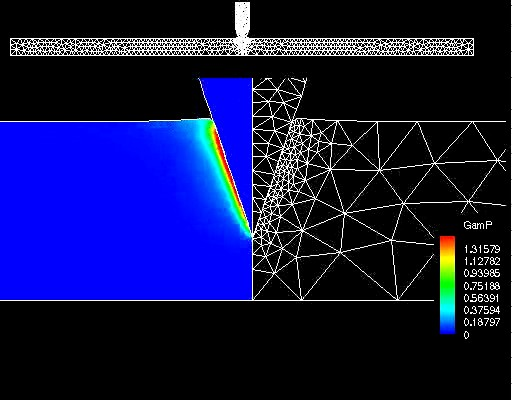
\includegraphics[width=0.5\textwidth,height=0.5\textheight]{./02-SECCION/Bala.jpg} 
  
  }{./02-SECCION/bala.mpg}
  \end{center}
\end{frame}


\subsection{Imágenes}
\begin{frame}{Imágenes}
  \begin{columns}
    \column{0.4\textwidth}
    \begin{beamercolorbox}[ht=20pt,wd=\textwidth,center,colsep=5pt]{highlight1}
      \centering Esta es una Imágen Simple \par
    \end{beamercolorbox}
    \column{0.5\textwidth}
    \begin{figure}
      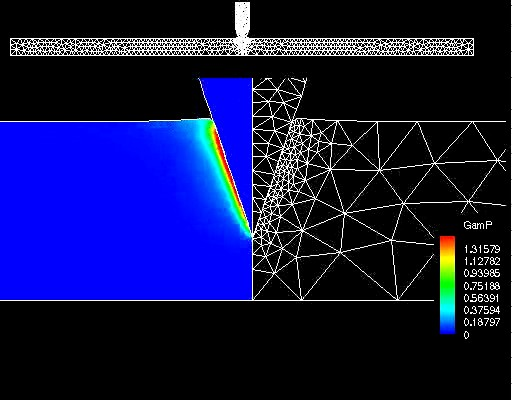
\includegraphics[width=\textwidth]{./02-SECCION/Bala.jpg}
      \caption{Influencia e importancia de la simulación en Ciencia de Materiales.}
    \end{figure}
  \end{columns}

\end{frame}


%\include{./02-SECCION/03-02-SECCION}

\section{Diapositivas con Slides}
\begin{frame}{Diapositivas con slides.}

  \begin{itemize}
    \item<1-> Individualizar el problema físico a estudiar: \\ \color{red} lo importante a tener en cuenta son las escalas tanto de tiempo como de distancias involucradas. \par 

      \item<2-> Desarrollar una \color{green} teoría y un modelo matemático  \color{black} para describir el fenómeno a estudiar.
      \item<3-> Llevar el modelo matemático a una forma manejable 
      \item<4-> por un programa de computación.
      \item<5-> Desarrollar o aplicar un algoritmo numérico para tratar 
      \item<6-> el modelo, compatible con su simulación.
      \item<7-> Escribir un código computacional que lo resuelva.
      \item<8-> Realizar el experimento computacional.
      \item<9-> Analizar los datos (mediante gráficos, tablas, curva, etc.).
      \item<10-> Iterar si hiciera falta! \color{green} (muchas veces!) \par  
  \end{itemize}
	\onslide<10-> \color{red} A menudo implica cambiar la forma de pensar un problema!!
\end{frame}


\section{Diapositivas con Notas}
\begin{frame}

\includegraphics[height=\textheight]{./02-SECCION/Clase-1.png} 

\note{
  Esta es una nota a la diapositiva, que debería 
  aparecer solo en la pantalla secundaria o bien
  al imprimir las notas. 
}

\note<1->{también se pueden usar notas en overlays}
\note<2->{como se ve aquí}

\end{frame}



\section{El Uso de recuadros}
\subsection{recuadros en el texto}


\begin{frame}{Recuadros simples alrededor del texto: tcolorbox}

  \begin{itemize}
  %% 
  \note{ \textbf{tcolorbox} parece ser la opcion más simple para estos casos }
  \note{ el comando \emph{ \\pause } genera slides! }
 \tcbset{colframe=blue,colback=white,width=\textwidth}
 \begin{tcolorbox}
      \item  Individualizar el problema físico a estudiar: \\ \color{red} lo importante a tener en cuenta son las escalas tanto de tiempo como de distancias involucradas. 
 \end{tcolorbox}
 \pause
      \item  Desarrollar una \color{green} teoría y un modelo matemático  \color{black} para describir el fenómeno a estudiar.
      \item  Llevar el modelo matemático a una forma manejable 
      \item  por un programa de computación.
      \item  Desarrollar o aplicar un algoritmo numérico para tratar 
      \item  el modelo, compatible con su simulación.
      \item  Escribir un código computacional que lo resuelva.
  \pause
  \note{ la posición de los tcolorbox se puede modificar asi: }
  \begin{tcolorbox}[enlarge left by=-0.1\textwidth , width=1.1\textwidth ]
      \item  Realizar el experimento computacional.
      \item  Analizar los datos (mediante gráficos, tablas, curva, etc.).
      \item   Iterar si hiciera falta! \color{green} (muchas veces!) \par  
  \end{tcolorbox}
  \pause
  \end{itemize}
  \color{red} A menudo implica cambiar la forma de pensar un problema!!

\end{frame}


\section{Diapositivas con tikz}
\begin{frame}{Una diapositiva con tikz}
\centering
%    \tikz[baseline] \node[anchor=base] (points) {\includegraphics[height=0.4\textheight]{./04-AJUSTE/FIG-DOTS.png}};
%    \tikz[baseline] \node[anchor=base] (interp) {\includegraphics[height=0.4\textheight]{./04-AJUSTE/FIG_SPLINE.png} };
%    \tikz \draw[->,thick,draw=blue] (points.west) -- (interp.east);
  \begin{tikzpicture}
    \node (points) at (-3,0) {\includegraphics[height=0.4\textheight]{./06-SECCION/FIG-DOTS.png}};
    \node (interp) at (3,0) {\includegraphics[height=0.4\textheight]{./06-SECCION/FIG_SPLINE.png} };
    \draw [->,>=latex,fill=blue!40!black,thick,draw=blue,line width=5pt] (points) -- (interp);
  \end{tikzpicture}
\vspace{1cm}
  \note con el paquete tikz es posible hacer graficas en la diapositiva, siendo posible evitar el uso de 
  imagenes externas. 
  \note problema es que cosas tan sencillas como la flecha pueden ser algo complicado de hacer. 
%    \tikz[baseline] \node[anchor=base] (points1) {\includegraphics[height=0.4\textheight]{./04-AJUSTE/FIG-DOTS.png}};
%    \tikz[baseline] \node[anchor=base] (interp1) {\includegraphics[height=0.4\textheight]{./04-AJUSTE/FIG_SPLINE.png} };
%    \begin{tikzpicture}[overlay,>=latex]
%      \path[blue,->] (points1) -- (interp);
%    \end{tikzpicture}

Existen muchos tipos de formas funcionales útiles para interpolar:
\begin{center}
\begin{itemize}
\item Polinomios
\item Funciones Trigonométricas
\item Exponenciales
\end{itemize}
\end{center}
\end{frame}
 
%\section{Conclusiones}
%\setbeamertemplate{background canvas}{
\includegraphics[width=\paperwidth,height=\paperheight]{/home/mariano/CuadernoTrabajo/CV/SLI/05-Conclusion/kitty.png}
}
\begin{frame}{\centering Such Experience, Much promise}
  \begin{itemize}
      \item Wide DFT experience gives me the tools to face all kind of difficult computational materials science 
	problems
      \item Experience in programming and linux system admininstration can give me a good insight in
	everyday work
      \item experience in interacting in multidisciplinary workgroups. 
  \end{itemize}


\end{frame}
\setbeamertemplate{background canvas}{}

\begin{frame}{Any Questions?}
\begin{center}
\resizebox{\textwidth}{0.8\textheight}{
\huge \textcolor{lightgray}{42}
}
\end{center}
\end{frame}


\end{document}
